% Szenarien und Annahmen

\section{Auswertung bestehender Literatur und Einordnung der Arbeit}\label{chap:Literatur}

In diesem Kapitel erfolgt eine Metaanalyse relevanter Studien, mit dem Fokus auf den getroffenen Annahmen zur Elektromobilität.
Bei den Studien, die sich explizit mit den Auswirkungen der Elektromobilität auf die Verteilnetze beschäftigen, werden zudem die verwendete Methodik und Ergebnisse betrachtet.


\subsection{Fahrzeughochlauf}

Aufgrund der zunehmenden Marktdurchdringung der Elektromobilität rückt die Frage der Rückwirkungen der Ladevorgänge auf die Stromnetze vermehrt in den Vordergrund.
Sind die Auswirkungen heutzutage noch klein, so kann ein stark steigender Markthochlauf auch starken Einfluss auf die Netzlast haben.
Neben der Anzahl an Fahrzeugen haben auch die technischen Parameter der einzelnen Fahrzeugklassen einen starken Einfluss.
Die verwendeten technischen Parameter der Fahrzeuge können \autoref{chap:EMob_Szenarien} entnommen werden.

\begin{figure}[H]
    \centering
    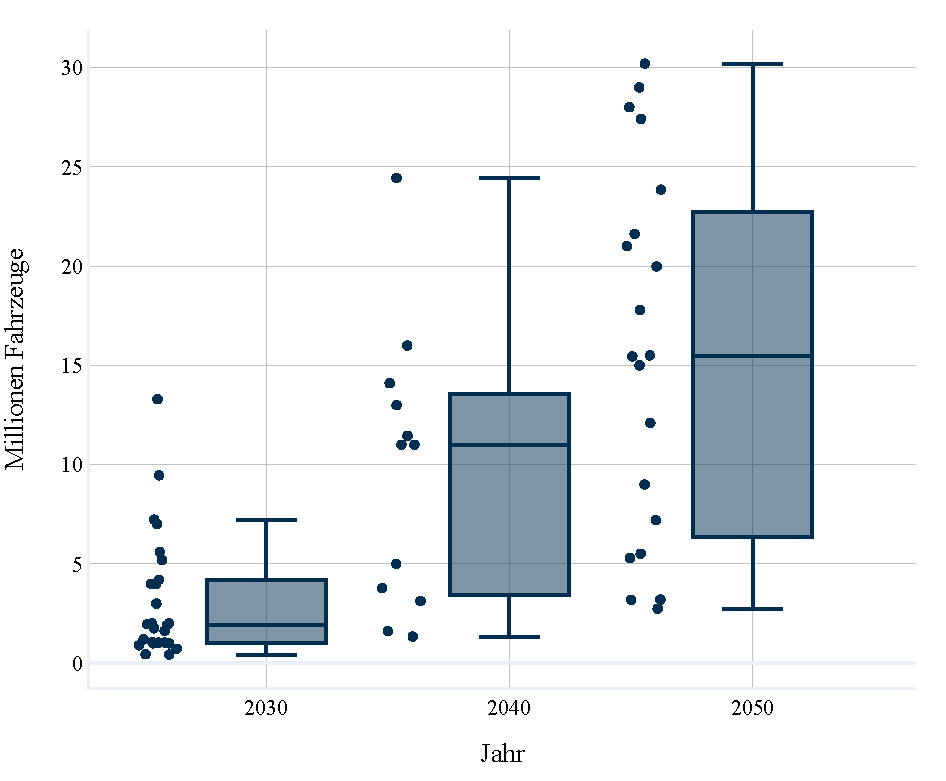
\includegraphics[width=\textwidth]{Bilder/RampUp-BEV-MA}
    \caption{Szenarienvergleich des Fahrzeugbestands von BEV bis zum Jahr \num{2050}}\label{fig:RampUpBEV}
\end{figure}

In \autoref{fig:RampUpBEV} sind die Annahmen der betrachteten Studien zum Fahrzeugbestand von \glspl{BEV} bis zum Jahr \num{2050} als Box-Plot dargestellt.
Die zugrundeliegenden Daten finden sich im Anhang in \autoref{tab:RampUpBEV}.
Trotz einer starken Streuung zeigt sich bis \num{2050} eine klare Zunahme des Bestandes.
Liegt der Median 2030 noch bei \SI{1.9}{\MioStk}, steigt dieser bis \num{2040} auf \SI{11.0}{\Mio} und erreicht \num{2050} \SI{15.5}{\Mio}.
Die starke Streuung lässt sich zum einen durch unterschiedliche Zielsetzungen der verschiedenen Studien und zum anderen durch den langen Zeithorizont und die damit verbundene Unsicherheit erklären.
In einzelnen Szenarien werden hohe Elektrifizierungsquoten angenommen und das Einhalten des \SIrange[range-phrase=~{--}~]{80}{95}{\percent}-Ziels des Klimaschutzplans \num{2050} vorausgesetzt, während andere Szenarien eine Fortschreibung der aktuellen Entwicklungen (\gls{BAU}) untersuchen.
So handelt es sich beispielsweise bei dem oberen Ausreißer im Jahr 2030 um das Elektrifizierungs-Szenario der dena-Leitstudie \textit{Integrierte Energiewende} \cite{DEAGH2018}.
Dieses nimmt hohe Elektrifizierungsquoten an setzt als Leitlinie die Einhaltung des \SIrange[range-phrase=~{--}~]{80}{95}{\percent}-Ziels.\medskip

Neben dem Hochlauf an \glspl{BEV}, ist auch mit einem starken Hochlauf bei den \glspl{PHEV} zu rechnen.
Da ein Großteil der Fahrten von \glspl{PKW} eine Strecke von \SI{50}{\km} nicht überschreiten \cite{Agora2019}, können viele Fahrten auch von \glspl{PHEV} batterieelektrisch zurückgelegt werden.

\begin{figure}[H]
    \centering
    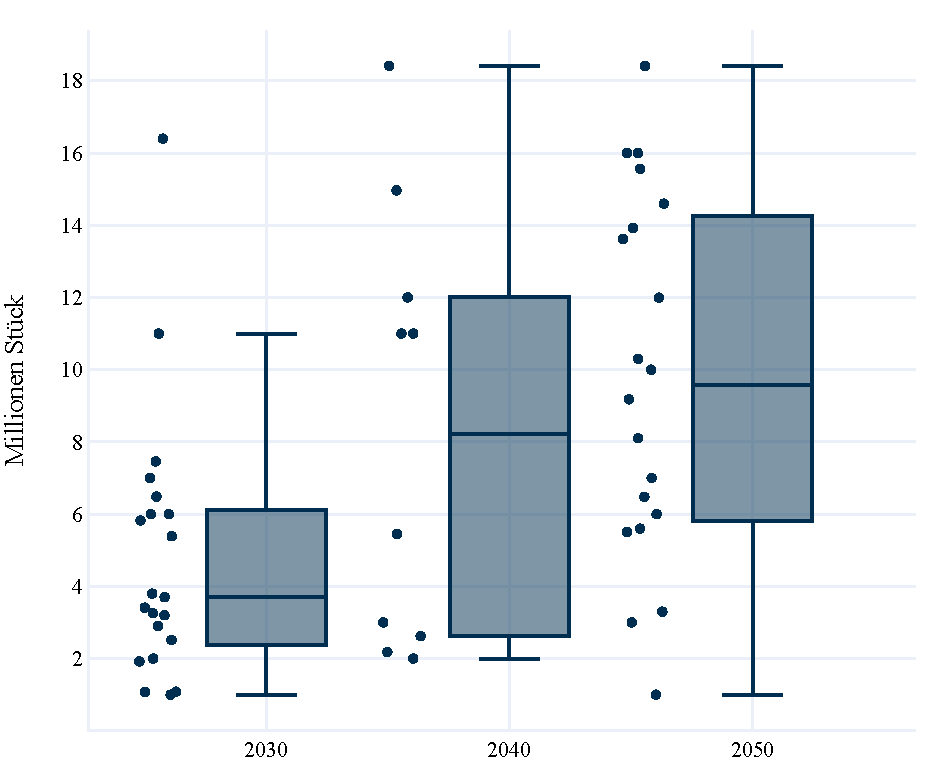
\includegraphics[width=\textwidth]{Bilder/RampUp-PHEV-MA}
    \caption{Szenarienvergleich des Fahrzeugbestands von PHEV bis zum Jahr \num{2050}}\label{fig:RampUpPHEV}
\end{figure}

\autoref{fig:RampUpPHEV} zeigt die Annahmen der betrachteten Studien zum Fahrzeugbestand von \glspl{PHEV} bis zum Jahr \num{2050} als Box-Plot.
Die zugrundeliegenden Daten finden sich im Anhang in \autoref{tab:RampUpPHEV}.
Bei \glspl{PHEV} liegt der Anstieg im Fahrzeugbestand anfangs sogar höher als bei \glspl{BEV}.
So liegt der Median 2030 bereits bei \SI{3.7}{\MioFZs}.
Anschließend fällt der Fahrzeugbestand von \glspl{PHEV} hinter den der \glspl{BEV} zurück.
Bis \num{2040} steigt dieser auf \SI{8.2}{\Mio} und \num{2050} auf \SI{9.6}{\MioStk}.
Je nach Studie und Szenario sinkt der Fahrzeugbestand nach \num{2040} sogar wieder, da zur Erreichung der Klimaziele oder aus ökonomischen Gründen der Umstieg auf \glspl{BEV} als sinnvoller eingeschätzt wird.


\subsection{Methodik zur Modellierung der Elektromobilität}

Von den betrachteten Studien quantifizieren drei Studien den Netzausbaubedarf auf Verteilnetzebene und besitzen somit einen Vergleichswert zu der vorliegenden Arbeit und werden vertieft betrachtet.
Hierzu zählen die dena-Leitstudie \textit{Integrierte Energiewende} \cite{DEAGH2018}, die BCG Studie \textit{Klimapfade für Deutschland} \cite{BCG2018} und die Agora Studie \textit{Verteilnetzausbau für die Energiewende} \cite{Agora2019}.

\begin{figure}[H]
    \centering
    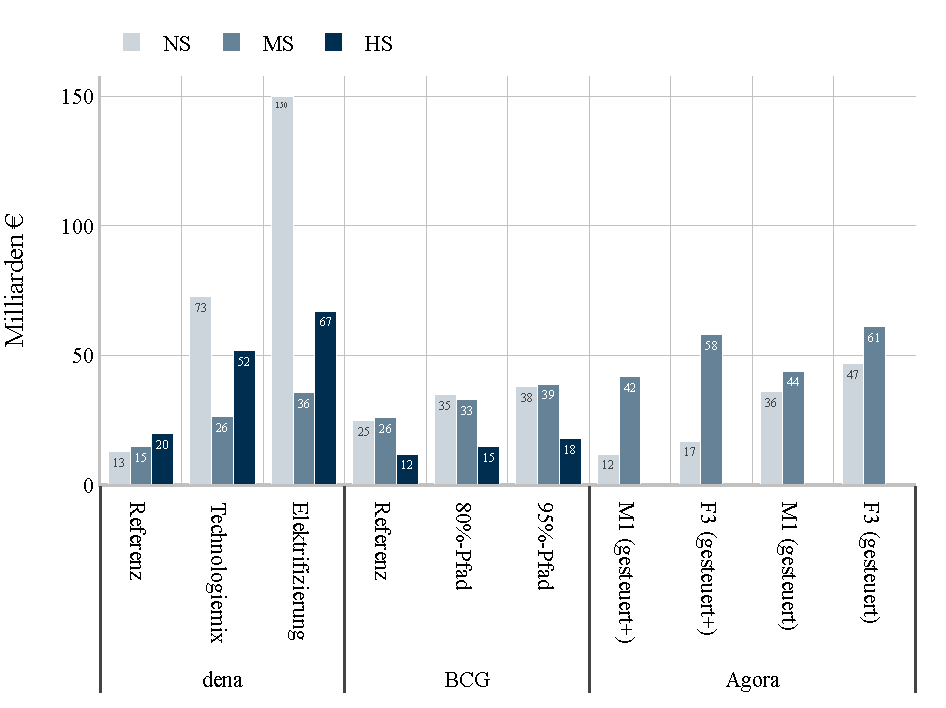
\includegraphics[width=\textwidth]{Bilder/DS-CAPEX-MA}
    \caption{Investitionsbedarf in die Verteilnetze bis zum Jahr \num{2050} je Spannungsebene}\label{fig:DSCAPEXMeta}
\end{figure}

In \autoref{fig:DSCAPEXMeta} werden die Ergebnisse der Studien für den Investitionsbedarf in die Verteilnetze bis zum Jahr \num{2050} aufgeteilt auf die drei Spannungsebenen \gls{NS}, \gls{MS} und \gls{HS} dargestellt.
Deutlich wird hierbei, dass die dena-Leitstudie die mit Abstand höchsten Kosten für den Netzausbau auf \gls{NS}- und \gls{HS}-Ebene ermittelt.
Die Agora Studie untersucht hingegen die Netzausbaukosten nicht auf der \gls{HS}-Ebene, ermittelt jedoch die höchsten Ausbaukosten aller Studien auf der \gls{MS}-Ebene.
Ein direkter Vergleich der Ergebnisse ist jedoch nur bedingt möglich, da die drei Studien unterschiedliche Grundsätze für ihre Szenarien und die Bestimmung des Netzausbaubedarfs ansetzen.
An dieser Stelle sollen deshalb die Unterschiede und Gemeinsamkeiten zwischen den drei Studien in der Methodik zur Einbindung von \glspl{EPKW} in das Netzmodell dargestellt werden.


\subsubsection{Bedarfsabschätzung}

Die Studien treffen bereits beim Hochlauf der Elektromobilität je Szenario stark unterschiedliche Annahmen, weshalb die Bedarfsabschätzung zwischen den Szenarien unterschiedlich ausfällt.
Die Zahlen für direktelektrifizierte Fahrzeuge in den ambitionierten Szenarien der Studien liegen mit minimal \SI{35}{\MioFZs} (BCG) und \SI{45}{\MioFZs} (Agora) allerdings in einer ähnlichen Dimension.
Der Verbrauch von \glspl{EPKW} wurde in der Agora Studie als homogen angenommen, während die dena-Leitstudie und die BCG Studie beim Verbrauch zwischen \glspl{BEV} und \glspl{PHEV} unterscheiden.
In der dena-Leitstudie und der BCG Studie wird eine Abschätzung der Veränderung im Mobilitätsverhalten vorgenommen, wodurch sich die Verkehrsleistung von \glspl{PKW} leicht verändert.
Demgegenüber wird bei der Agora Studie keine Veränderung der Verkehrsleistung gegenüber dem heutigen Stand angenommen.
Die Abschätzung der lokalen Belastungen durch die Elektromobilität erfolgt innerhalb der dena-Leitstudie und der Agora Studie anhand einer Evaluierung der Gleichzeitigkeit in Abhängigkeit vom Ladeort und der Anzahl der Fahrzeuge.
Die Evaluierung der Gleichzeitigkeit erfolgt in beiden Fällen anhand einer Monte-Carlo-Simulation simulierter Lastgänge, wobei das \SI{95}{\percent}-Quantil als auslegungsrelevant für die Netzplanung angesehen wird.
Die Agora Studie erweitert diese Annahme um die Abhängigkeit der Gleichzeitigkeit von der Ladeleistung.


\subsubsection{Ladestrategien}

Ein deutlicher Unterschied entsteht durch die Annahme der dena-Leitstudie, dass eine Steuerung der Ladevorgänge von neuen Verbrauchern nicht stattfindet.
Stattdessen geht die Studie davon aus, dass die zusätzliche Last durch \glspl{EPKW} und \glspl{WP} gleichzeitig mit der bisherigen Spitzenlast auftritt und der auslegungsrelevante Starklastfall somit deutlich erhöht wird.
Im Gegensatz zur dena-Leitstudie wird in der BCG-Studie von einem gesteuerten Laden der neuen Verbraucher ausgegangen.
Hierbei reagieren \SI{80}{\percent} der \glspl{EPKW} auf Strommarktsignale und werden nur geladen, wenn der \gls{SOC} auf weniger als \SI{50}{\percent} fällt oder eine lange Fahrt ansteht.
Bei der Agora Studie wird ein starker Fokus auf den Einfluss von aktiven netzdienlichen Ladestrategien auf den Netzausbaubedarf gelegt, indem eine Residuallastglättung innerhalb eines Netzgebietes angestrebt wird (gesteuert).
Ergänzend wurde ein erweitertes netzdienliches Ladekonzept (gesteuert\Plusdot) untersucht, welches zusätzlich zur Residuallastglättung die Verschiebung der Ladevorgänge über mehrere Standzeiten und eine Kappung von Lastspitzen erlaubt.
Das gesteuerte und gesteuert\Plus Laden werden in Form eines Reduktionsfaktors in der Netzplanung berücksichtigt.


\subsection{Abgrenzung zur vorliegenden Literatur}

In der ausgewerteten Literatur werden die Auswirkungen einer zunehmenden Netzintegration von \glspl{EPKW} auf die Verteilnetze in Deutschland bereits in ihrer Gesamtheit betrachtet.
In dieser Arbeit werden ergänzend die Auswirkungen auf fünf konkrete Referenznetzgebiete untersucht, welche jeweils stark unterschiedliche Charakteristika besitzen und grob in die Kategorien \gls{PV}-, Wind- bzw. Last-dominiert eingeteilt werden können.
Hierbei wird der Einfluss verschiedener netzdienlicher Ladestrategien untersucht und der Erfolg von präventiven und aktiven Ansätzen miteinander verglichen.
Somit soll eine Aussage darüber möglich werden, ob aktive Ansätze gegenüber präventiven Ansätzen einen wesentlichen Vorteil bieten.\medskip

In dieser Arbeit soll erweiternd zur vorliegenden Literatur ein verstärkter Fokus auf eine detaillierte Modellierung des Fahrzeugbestandes mit verschiedenen Fahrzeugklassen von \glspl{EPKW} gelegt werden.
Weiterhin werden für die Untersuchung der Auswirkungen auf die Verteilnetze nicht feste Gleichzeitigkeiten und Reduktionsfaktoren ermittelt, sondern konkrete Bedarfszeitreihen verwendet.


\clearpage
